%%%%%%%%%%%%%%%%%%%%%%%%%%%%%%%%%%%%%%%%%%%%%%%%%%%%%%%%%%%%%%%%%%%%%%%%%%%%%%%%
% ↓ pandoc stuff
% Options for packages loaded elsewhere
\PassOptionsToPackage{unicode}{hyperref}
\PassOptionsToPackage{hyphens}{url}
%
\documentclass[
  12pt
]{article}
\usepackage{amsmath,amssymb}
\usepackage{iftex}
\usepackage[a4paper]{geometry}
\ifPDFTeX
  \usepackage[T1]{fontenc}
  \usepackage[utf8]{inputenc}
  \usepackage{textcomp} % provide euro and other symbols
\else % if luatex or xetex
  \usepackage{unicode-math} % this also loads fontspec
  \defaultfontfeatures{Scale=MatchLowercase}
  \defaultfontfeatures[\rmfamily]{Ligatures=TeX,Scale=1}
\fi
\usepackage{lmodern}
\ifPDFTeX\else
  % xetex/luatex font selection
\fi
% Use upquote if available, for straight quotes in verbatim environments
\IfFileExists{upquote.sty}{\usepackage{upquote}}{}
\IfFileExists{microtype.sty}{% use microtype if available
  \usepackage[]{microtype}
  \UseMicrotypeSet[protrusion]{basicmath} % disable protrusion for tt fonts
}{}
\makeatletter
\@ifundefined{KOMAClassName}{% if non-KOMA class
  \IfFileExists{parskip.sty}{%
    \usepackage{parskip}
  }{% else
    \setlength{\parindent}{0pt}
    \setlength{\parskip}{6pt plus 2pt minus 1pt}}
}{% if KOMA class
  \KOMAoptions{parskip=half}}
\makeatother
\usepackage{xcolor}
\setlength{\emergencystretch}{3em} % prevent overfull lines
\providecommand{\tightlist}{%
  \setlength{\itemsep}{0pt}\setlength{\parskip}{0pt}}
% \setcounter{secnumdepth}{-\maxdimen} % remove section numbering % TODO: Corr: this is where most of the numbering fuckups come from.
\ifLuaTeX
  \usepackage{selnolig}  % disable illegal ligatures
\fi

%%%%%%%%%%%%%%%%%%%%%%%%%%%%%%%%%%%%%%%%%%%%%%%%%%%%%%%%%%%%%%%%%%%%%%%%%%%%%%%%
% ↓ Theorem styles

\usepackage{mathrsfs}
% \usepackage{amsthm}
% \usepackage{thm-amsthm}
\usepackage[standard,amsmath,thref,hyperref]{ntheorem}
\theorempreskip{20pt} % TODO: hacky
\theorempostskip{10pt} % TODO: hacky
\theoremstyle{break}
\theorembodyfont{\normalfont}
\newtheorem{thm}{Theorem}[section]
\newtheorem{defn}{Definition}[thm]
\newtheorem*{problem}{Problem}
\theoremstyle{plain}
\newtheorem{lem}[thm]{Lemma}
\newtheorem{prop}[thm]{Proposition}
\newtheorem{cor}[thm]{Corollary}
\newtheorem*{pf}{proof}
\theoremindent1cm
\newtheorem*{rk}{Remark}
\newtheorem*{ex}{Example}





\IfFileExists{bookmark.sty}{% if bookmark
  \usepackage{bookmark}
}{% else
\usepackage[
  colorlinks,
  citecolor=blue,
  filecolor=blue,
  linkcolor=blue,
  urlcolor=blue
]{hyperref}}
\IfFileExists{xurl.sty}{\usepackage{xurl}}{} % add URL line breaks if available
\urlstyle{same}

% ↑ from pandoc

%%%%%%%%%%%%%%%%%%%%%%%%%%%%%%%%%%%%%%%%%%%%%%%%%%%%%%%%%%%%%%%%%%%%%%%%%%%%%%%%
% ↓ custom commands

% I'm lazy
\usepackage{xspace}
\newcommand{\G}{\ensuremath{G}\xspace}
\newcommand{\Gamm}{\ensuremath{\Gamma}\xspace}
\newcommand{\mpi}{\ensuremath{\pi}\xspace}

% special typefaces
\newcommand{\bbr}{\ensuremath{\mathbb{R}}\xspace}
\newcommand{\bbc}{\ensuremath{\mathbb{C}}\xspace}
\newcommand{\hilb}{\ensuremath{\mathscr{H}}\xspace}

% my favorite spaces
\newcommand{\sltr}{\ensuremath{SL(2, \mathbb{R})}\xspace}
\newcommand{\slnr}{\ensuremath{SL(n, \mathbb{R})}\xspace}

\newcommand{\frg}{\ensuremath{\mathfrak{g}}\xspace}
\newcommand{\frk}{\ensuremath{\mathfrak{k}}\xspace}
\newcommand{\fra}{\ensuremath{\mathfrak{a}}\xspace}
\newcommand{\frnn}{\ensuremath{\mathfrak{n}}\xspace}

% inline matrix. why was this removed??
\newcommand{\ipmatrix}[1]{%% make inline smallmatrix with parens. suited for 2x2 matrices.
\ensuremath{\big(\begin{smallmatrix} #1 \end{smallmatrix}\big)}\xspace}
\newcommand{\Ginv}{{\ensuremath G}-invariant}
\newcommand{\Ninv}{{\ensuremath N}-invariant}

% surrounding marks
\newcommand{\abs}[1]{| #1 |}
\newcommand{\inn}[1]{\left\langle #1 \right\rangle}
\newcommand{\norm}[1]{\lVert #1 \rVert}

% operators
\DeclareMathOperator{\Aut}{Aut}
\DeclareMathOperator{\Id}{Id}
\DeclareMathOperator{\id}{id}

%%%%%%%%%%%%%%%%%%%%%%%%%%%%%%%%%%%%%%%%%%%%%%%%%%%%%%%%%%%%%%%%%%%%%%%%%%%%%%%%
% ↓ bibtex stuff

\usepackage{biblatex}
\addbibresource{refs.bib}

%%%%%%%%%%%%%%%%%%%%%%%%%%%%%%%%%%%%%%%%%%%%%%%%%%%%%%%%%%%%%%%%%%%%%%%%%%%%%%%%
% ↓ images

\usepackage{graphicx}
\usepackage{svg}

%%%%%%%%%%%%%%%%%%%%%%%%%%%%%%%%%%%%%%%%%%%%%%%%%%%%%%%%%%%%%%%%%%%%%%%%%%%%%%%%
% ↓ declaration of originality

\usepackage{pdfpages}

%%%%%%%%%%%%%%%%%%%%%%%%%%%%%%%%%%%%%%%%%%%%%%%%%%%%%%%%%%%%%%%%%%%%%%%%%%%%%%%%
% ↓ document

% \usepackage{lineno}
% \linenumbers


\hypersetup{
  pdftitle={On Theorem by Moore about Vanishing Matrix Coefficients},
  pdfauthor={Nicolas Trutmann},
  % hidelinks,
  pdfcreator = {Nicolas Trutmann},
  pdfkeywords = {Ergodic Theory},
}

\title{On Theorem by Moore about Vanishing Matrix Coefficients}
\author{Nicolas Trutmann}
\date{}

%%%%%%%%%%%%%%%%%%%%%%%%%%%%%%%%%%%%%%%%%%%%%%%%%%%%%%%%%%%%%%%%%%%%%%%%%%%%%%%%

\begin{document}
\maketitle

\begin{abstract}
  In this paper we will showcase a theorem in ergodic theory by R. Howe and
  C.C. Moore \cite{howe79}, as it is presented in the book by R.J. Zimmer in his
  book "\citetitle{Zimmer84}" \cite{Zimmer84}.
  % TODO: is this actually the right citation?
  On the way there, we will touch many different
  fields, from measure theory, over functional analysis, representation
  theory and of course ergodic theory.
\end{abstract}

\newpage
\tableofcontents
\newpage


  This paper is based on the first two chapters in the book ``Ergodic Theory
  and semisimple Lie Groups'' by Robert Zimmer \cite{Zimmer84}, which contain
  the theorem itself (Theorem 2.2.20), which we will state shortly, and
  surrounding material concerning ergodic theory.

  The techniques of the proof show a nice interplay between fields and
  their different approaches, while staying relatively simple. We assume
  the reader to have an undergraduate level understanding of the
  prerequisites in algebra and representation theory, but will state
  foundational information regardless, and provide references in all
  cases. We also take care of clarifying notation before use.

  The theorem is historically at home in the
  development of ergodic theory, which in turn is a relatively new field
  of mathematics. The original definition of ergodicity was given in 1928
  in a paper by P. Smith and G.D. Birkhoff on dynamical systems. The concept
  gained importance in 1931 when von Neumann and Birkhoff nearly
  simultaneously proved the mean and pointwise ergodic theorems. These may
  be regarded as the starting point of the subject.

  The theory presented here is almost entirely due to a single mathematical
  lineage. The root of this lineage is George David Birkhoff, who, on one side was the
  (biological) father of Garrett Birkhoff, which in turn was the advisor of G. Mostow,
  known for his rigidity theory which was instrumental to G. Margulis' rigidity
  and arithmeticity theorem. These theorems are a central part of Zimmer's book,
  although we will not cover them. On the other side, G.D. Birkhoff was 
  M.H. Stone's advisor who was G. Mackey's advisor, whose work on representations will
  feature prominently in the chapter \hyperlink{the-direct-integral-and-unitary-representations}{on unitary representations}.
  And Mackey was the advisor of R.J. Zimmer, the author of our main reference, as
  well as C.C. Moore, who, together with his student R. Howe, worked out the
  theorem we are talking about in this paper.

  To give an extremely rough idea of the subject, classical ergodic theory concerns itself with (group) actions on some (measure) space
  describing long-term behavior of dynamical systems.
  The classical example comes from thermodynamics. Consider the motion of particles in an ideal gas.
  Ergodicity provides a framework for studying the common-sense notion that the particles would eventually mix completely (i.e. reach every possible configuration of the space),
  like smoke in an enclosed room would eventually fill the entire room completely.

  The way this behavior is modelled is by a time evolution map $T:X \rightarrow X$ on some phase space $X$,
  and ergodicity is expressed in the following way :

  There is no proper subset of $X$, $\emptyset \subsetneq A \subsetneq X$ that is also invariant with respect to some measure $\mu$,
  meaning there is no proper subset such that $\mu(A) = \mu(TA)$.
  Equivalently, if $A$ is invariant then either $\mu(A) =0$ ($A$ is a null set) or $\mu(A) = \mu(X)$.

  Mathematicians found purely mathematical interest in this behavior and began studying it on its own,\
  dropping the physical notion of configuration space and time evolution and substituting the evolution map with group actions $G:X \rightarrow X$.
  Notably using topological groups such as Lie groups, as we will do in this paper.

  The main aim of the book by Zimmer is focused on two theorems by Mostow and
  Margulis. The ``arithmeticity theorem'' and the ``rigidity theorem'', which
  show how Lie groups and their lattices interact. 

  A lattice \Gamm in a locally compact topological group \G is a discrete subgroup such that the quotient $G/\Gamma$ has finite invariant measure.
  For example, $\mathbb{Z}^n$ in $\bbr^n$ is a lattice, as is $SL(n, \mathbb{Z})$ in $\slnr$.
  The rigidity and arithmeticity theorems state (very roughly) that lattices determine the surrounding group and groups determine lattices.
  This glosses over a tremendous amount of detail, but these theorems are not the focus of this paper, so this shall suffice.
  They serve the purpose of motivating the study of lattices in Lie groups.



%%%%%%%%%%%%%%%%%%%%%%%%%%%%%%%%%%%%%%%%%%%%%%%%%%%%%%%%%%%%%%%%%%%%%%%%%%%%%%%%%%%%%%%%%%%%%%%%%%%%


\hypertarget{introduction}{\section{Introduction}\label{sec:introduction}}

  We should, at this point, introduce the theorem we would like to present.

  In \citeauthor{Zimmer84}\cite{Zimmer84} it is Theorem 2.2.20, and originally from \citeauthor{howe79}\cite{howe79}.

  \begin{thm}[Howe-Moore's Ergodicity Theorem]
    \label{thm:main-thm}
    Let $G_i$ be connected non-compact simple Lie groups with finite center, $G = \prod G_i$ and $\pi$ a unitary representation of \G.
    Then all matrix coefficients $f(g) = \inn{\pi(g)v,w}$ vanish at infinity.
    I.e. $f(g) \rightarrow 0$ as $g$ leaves compact subsets of \G.
  \end{thm}

  To clarify some points, note that we have specified non-compact groups.
  This allows us to talk about ``infinity'' at all. Next, what is an
  invariant vector? Simply, a vector $v$ is called invariant if for all $g\in G$
  $\pi(g)v = v$, or, that $v$ is preserved by any linear map
  given by the representation.

  \hypertarget{question-when-is-an-action-ergodic}{%
  \subsection{Question: when is an action
  ergodic?}\label{question-when-is-an-action-ergodic}}

  Instead of verifying ergodicity for any given action, space and measure
  individually, can we find criteria for ergodicity that are easier to
  evaluate? Moore's theorem sits in the middle of an argument that
  answers the following questions.

  For example, consider a group \G, a lattice $\Gamma \subset G$ and a closed subgroup $H \subset G$.
  this is of course, a priori, a bit of a contrived example, but consider that lattices in Lie groups are a considerable field of study.

  \begin{problem}[When do closed subgroups act ergodically]
    If $H_1, H_2 \subset G$ are closed subgroups in \G, is the action $H_1\curvearrowright G/H_2$ ergodic?
  \end{problem}

  \begin{problem}[When do closed subgroups act ergodically]
    Let \G be a semisimple Lie group and $S$ an ergodic \G-space. If $H\subset G$ is a closed subgroup, when is $H$ ergodic on $S$.
  \end{problem}


  Now that we have a concrete question, let us try to get our hands dirty
  on an example. We will consider the action of fractional linear transforms on
  the upper half plane
  It will bring intuition about the question and why one would care to
  answer the question.

  Let $X = \{z \in \bbc  | Im(z) >0\}$ be the upper half plane, and $G = \sltr$.
  \G acts on $X$ via fractional linear transformations, i.e.
  $$
  g \cdot y = (ay + b)/(cy +d) \text{ where } g= \begin{pmatrix}
    a & b \\
    c & d 
  \end{pmatrix}
  $$

  We would like to understand the actions of a lattice in \G on $X$.

  Suppose now $\Gamma \in G$ is a lattice. 
  If $G$ acts transitively on a space $X$, then there is an isomorphism
  of $G$-spaces $G/G_x \rightarrow X$, where $G_x = Stab_G (x)$ for
  $x \in X$, given by the map $gG_x \mapsto gx$. In the case of our
  example $G = SL(2, \mathbb{R})$

  the stabilizer of $i$ to be $SO(2,\mathbb{R})$.
  We want to show that the action of $\Gamma$ on
  $\bar{\mathbb{R}} = \bbr \cup \{\infty\}$ is ergodic.

  \begin{defn}[Ergodicity]
    Let \G be a locally compact second countable group.
    We consider actions of \G on a measure space $(S, \mu)$, where $\mu$ is
    $\sigma$-finite and quasi-invariant under the action of \G.
    \emph{Quasi-invariant} means that for all set $A \subset S$ and $g \in G$,
    $\mu(A) = 0$ if and only if $\mu(gA) = 0$.

    For such \G, $(S, \mu)$ an action $G \times S \rightarrow S$ is called
    ergodic if all $G$-invariant subsets $A\subset S$ are either null or
    conull.
    Which means 
    $$
    \forall g\in G:\ gA = A \quad \Rightarrow \quad \mu(A)=0 \text{ or } \mu(S\setminus A)=0
    $$
  \end{defn}

  % TODO: unoriginal

  Since the action of $G$ on $X$
  allows an identification of $X$ with $G/K$, where $K = SO(2)$ (the
  stabilizer of $i \in X$), and $K$ is compact, it follows that the
  action of $\Gamma$ on $X$ is properly discontinuous, and so
  $\Gamma\backslash X$ will be a manifold, in fact a finite volume
  Riemann surface.

  On the other hand, via the same fractional linear transformation
  formula, $G$ acts on
  $\bar{\mathbb{R}} = \mathbb{R} \cup \{ \infty \}$, and
  $\bar{\mathbb{R}}$ can be identified with $G/P$, where $P$ is the
  group of upper triangular matrices and the stabilizer of
  $\infty \in \bar{\mathbb{R}}$. Once again, we can consider the action
  of $\Gamma$ on $\bar{\mathbb{R}}$, but now the action will be very
  far from being properly discontinuous. In fact, every $\Gamma$-orbit
  in $\bar{\mathbb{R}}$ will be a (countable) dense set. In particular,
  if we try taking the quotient $\Gamma\backslash\bar{\mathbb{R}}$, we
  obtain a space with the trivial topology. On the other hand,
  $\bar{\mathbb{R}}$ provides a natural compactification of $X$, and
  in fact $\bar{\mathbb{R}}$ can be identified with asymptotic
  equivalence classes of geodesics in $X$, where $X$ has the
  essentially unique $G$-invariant metric.


%%%%%%%%%%%%%%%%%%%%%%%%%%%%%%%%%%%%%%%%%%%%%%%%%%%%%%%%%%%%%%%%%%%%%%%%%%%%%%%%%%%%%%%%%%%%%%%%%%%%


\hypertarget{definitions-and-notation}{%
\section{Definitions and Notation}\label{definitions-and-notation}}


  Now that we have stated the goal of the paper, let us immediately make a
  detour. We will state definitions and relevant theorems (without proof)
  in compact form with ample references so that a reader can catch up if
  necessary. The advanced reader can skip this section and move straight
  to the \hyperref[the-direct-integral-and-unitary-representations]{next topic} without issue.

  % TODO:  (put references for everything in each section)
  % Throughout the whole text, unless otherwise stated, G is a countable
  % discrete group. Its identity element will always be denoted by e.



  \hypertarget{measure-spaces}{%
  \subsection{Measure Spaces}\label{measure-spaces}}

  A \emph{measurable space} is a pair $(X, \mathscr{B})$ where $X$ is
  a set and $\mathscr{B}$ is a $\sigma$-algebra of subsets of $X$.
  Elements of $\mathscr{B}$ are called \emph{measurable sets}. A
  function of measurable spaces $f: X \rightarrow Y$ is called
  \emph{measurable} if $f^{-1}(A)$ is a measurable set in $X$ for all
  measurable sets $A$ of $Y$.

  The Borel $\sigma$-algebra of a topological space $X$ is the
  $\sigma$-algebra $\mathscr{B}$ generated by the open subsets of
  $X$ , and the members of $\mathscr{B}$ are called Borel sets. 

  A \emph{measure} on a measurable space $(X, \mathscr{B})$ is a map
  $\mu: \mathscr{B} \rightarrow [0, \infty]$ such that
  \begin{itemize}
    \item $\mu(\emptyset) = 0$, and
    \item $\mu(\cup_{n=1}^{\infty} A_n) = \sum_{n=1}^{\infty} \mu(A_n)$ 
  \end{itemize}
  for
  every countable collection $\{A_n\}_{n=1}^{\infty}$ of pairwise
  disjoint sets in $\mathscr{B}$ (countable additivity).

  A measure $\mu$ is called \emph{finite} if the whole space has finite measure $\mu(X) < \infty $,
  and \emph{$\sigma$-finite} if $X$ is the countable union of sets with finite measure,
  meaning, there exist sets $\{A_i\}_{i\in \mathbb{N}}$ such that $\cup_{i=1}^{\infty} A_i = X$ and
  $\mu(A_i) < \infty $ for all $i$.


  \hypertarget{groups}{%
  \subsection{Groups}\label{groups}}

  We are interested in Lie groups. Primarily for their nature as a topological group.
  A \emph{ Lie group } is a group that is also a manifold. A \emph{locally compact} group
  is locally compact as a topological space.
  We require groups to be locally compact, so that the Haar measure exists, which is, up to scaling,
  the unique measure on Borel sets which satisfies the following: For all $g\in G$
  $\mu(gS) = \mu(S)$, $\mu$ is finite on compact sets and is inner and outer
  regular.

  A \emph{lattice} is an invariant discrete subgroup $\Gamma$ of a locally
  compact group $G$ such that there exists a finite measure on the quotient
  space $G/\Gamma$.


  \hypertarget{group-actions}{
  \subsection{Group Actions}\label{group-actions}}

  By an \emph{action} of the group $G$ on a set $X$ we mean a
  map $\alpha: G \times X \rightarrow X$ such that, writing the first
  argument as a subscript, $\alpha_s(\alpha_t(x)) = \alpha_{st}(x)$ and
  $\alpha_e(x) = x$ for all $x \in X$ and $s, t \in G$.
  Most of the time we will not give this map a name and write the image of a pair
  $(s, x)$ written as $sx$. For sets $A \subset X$ and $K \subset G$
  and an $s \in G$ we write
  $$
  s A = \{sx : x \in A\},
  \quad
  K x = \{sx : s \in K \},
  \quad
  K A = \{sx : x \in A \text{ and } s \in K \}.
  $$
  The \emph{G-orbit} of a point $x \in X$ is the set $Gx$.

  \hypertarget{representations}{%
  \subsection{Representations}\label{representations}}

  % TODO: matrix coefficients

  A \emph{representation} is a group-homomorphism from a group into the general linear
  group of a vector space, $\pi: G \rightarrow GL(V)$.
  We consistently use lowercase Greek letters to refer to representations.
  Most often $\pi$.
  The \emph{dimension} of a representation is the dimension of the vector space
  that is being represented onto.


  A \emph{unitary operator} on a Hilbert space \hilb is a bounded linear
  operator $U$, such that $U^*U= UU^* = \Id_{\hilb}$. A \emph{unitary
  representation} is a representation into the unitary group of a vector space
  $\pi: G \rightarrow \mathcal{U}(V) \subset GL(V)$, where the unitary group
  consists of all unitary operators on \hilb.

  For a representation $\pi$ onto a (complex) Hilbert space \hilb, $\pi:G \rightarrow GL(\hilb)$
  and two vectors $v, w \in \hilb$,
  a \emph{matrix coefficient} is a map $f(g): G \rightarrow \bbc$ defined by
  $$
  f(g) = \inn{\pi(g)v, w}
  $$
  In the case of a finite dimensional Hilbert space and, for a given choice of basis, and two basis vectors $e_i,\ e_j$,
  the inner product $\inn{e_i\pi(g), e_j}$ works out to be the coefficient of the matrix associates to $\pi(g)$.


  % TODO: (all of this) repr: a map dim of a repr
  % TODO: agree with topology.




  \hypertarget{direct-difference-notation}{%
  \subsection{``Direct difference''
  notation}\label{direct-difference-notation}}

  Zimmer, and we, use the symbol ``$\ominus$'' to denote ``subtraction''
  of linear subspaces of Hilbert spaces. If $A \subset B$ are linear
  subspaces of a Hilbert space,
  $B \ominus A = \{x \in B: (x,y) = 0 \text{ for all }y \in A\}$.

  The specifically we will use it on $L^2(\hilb) \ominus \bbc$, to denote
  the square integrable functions on \hilb "minus" the subspace of constant functions.


  \hypertarget{ergodicity}{%
  \subsection{Ergodicity}\label{ergodicity}}

  % \begin{defn}{quasi-invariant}
  % A measure $\mu$ is quasi-invariant under a group action of $G$ if it preserves null sets.
  % If $A = gA$ then either $\mu(A)=0$ or $\mu(S\setminus A)=0$.
  % \end{defn}

  We have successfully made our way back to ergodicity. We will try to
  illuminate the definition a bit by examples and non-examples.

  To reiterate % TODO: have we iterated it once?

  \begin{defn}{Ergodicity}
  For a group $G$, a measurable separable space $S$, and a $G$-invariant
  measure $\mu$. An action is called ergodic if all $G$-invariant subsets
  $A\subset S$ are either null or conull. Which means
  $$
  \forall g\in G:\ gA = A \quad \Rightarrow \quad \mu(A)=0 \text{ or }
  \mu(S\setminus A)=0
  $$
  \end{defn}

  Let us try to build some intuition for what this means. Notice that orbits
  are, by definition \Ginv, so one way to constructively build invariant sets
  is to consider orbits of actions. Inversely as well, any invariant set can be
  considered a union of orbits of all its points. Recall from basic group
  theory that orbits partition the space, so saying that these must be either
  null or conull means there is no straightforward ``divide and conquer''
  strategy for understanding ergodic actions. In this regard ergodicity
  resembles a sort of ``irreducibility''-property. To put it in Zimmer's words
  ``Ergodic theory is (in large part) the study of complicated orbit structure
  in the presence of a measure.''


  Note, that the adjective ``ergodic'' sometimes applied to either the action, the measure or the space.
  What that means is that, for two out of three given, the third completes the definition.
  All three are necessary to be ergodic but when, for example, we have a group
  action on a space, we call a measure ergodic if together with the others they
  are ergodic.


  \begin{ex}
    Let $\mathbb{T}$ be the circle group of $\{z\ \bbc \ | \ |z| = 1 \}$ and
    $A: \mathbb{T} \rightarrow \mathbb{T}$ multiplication by $e^{i\alpha}$ with
    $\alpha/2\pi$ irrational. This induces an action
    $\mathbb{Z}\curvearrowright\mathbb{T} \rightarrow \mathbb{T}$ by $ n\cdot z
    \mapsto e^{in\alpha}z$. As a measure we take the arc-length measure, which
    is preserved under the action of $A$.

    This is an example of an ergodic action.

    To prove this, suppose $S \subset \mathbb{T}$ is $A$-invariant. We take
    $\chi_S(z) = 1 \text{ for } z\in S \text{ and } 0 \text{ for } z \notin S$,
    the characteristic function of $S$ and take the $L^2$-Fourier expansion
    $\sum a_n z^n$. Then, by invariance, $\chi_S(z) = \chi_S(e^{i\alpha}z) =
    \sum a_n e^{in\alpha}z^n$. Therefore $a_ne^{in\alpha} = a_n$. By assumption
    $\alpha/2\pi \notin \mathbb{Q}$, so $a_n = 0$ for all $n \neq 0$. This
    implies $\chi_S$ is constant, meaning either constant $0$ or constant $1$,
    which implies ergodicity.
  \end{ex}


%%%%%%%%%%%%%%%%%%%%%%%%%%%%%%%%%%%%%%%%%%%%%%%%%%%%%%%%%%%%%%%%%%%%%%%%%%%%%%%%


\hypertarget{the-direct-integral-and-unitary-representations}{%
\section{The Direct Integral and Unitary Representations}\label{the-direct-integral-and-unitary-representations}}


  Now that we've laid out the prerequisites, we can turn to what we'll actually need in terms of this specific subject.
  We have to take a detour into unitary
  representations and define the direct integral to make statements about
  certain subgroups, in particular $\bbr^n$.
  It turns out, we can transform questions about ergodicity into questions about representations.
  Thereby opening up the problems to more tractable linear algebra and matrix groups.

  The question about ergodicity, that hangs in the background of the theorem is:
  ``what happens at the boundary?''. Boundary means we are interested in the limit behavior of an ergodic action, which explains why our theorem makes an assertion about matrix coefficients at infinity.

  The way there will lead us through the direct integral, unitary representations
  and in particular the representation of $\mathbb{R}^n$. To jump ahead of
  ourselves, we'll later look at the upper diagonal group and its subgroup
  \ipmatrix{1 & x \\ 0 & 1}, which is isomorphic to $\mathbb{R}$ and whose
  representation we'll care about.

  \hypertarget{the-direct-integral}{%
  \subsection{The Direct Integral}\label{the-direct-integral}}

  In simple terms, the direct integral is a way to patch together locally
  defined functions into a function on the whole domain. Let us first
  consider the simple case where we have global functions on a measure
  space $M$, that takes values in some Hilbert space $\mathscr{H}$,
  $f:M \rightarrow \mathscr{H}$. The `sensible' space to put these
  functions into is the space of square integrable functions on $M$,
  denoted $L^2(M, \mathscr{H})$. The word `sensible' here is justified
  by being again a Hilbert space by integration
  $\langle f, g\rangle = \int_M\langle f(x), g(x)\rangle$.

  % TODO:  (doesn't mention measurablity)

  The next step towards locality is to use two function, by defining
  $L^2(M_1 \sqcup M_2, \mathscr{H}_1 \oplus \mathscr{H}_2)$, where every
  function is defined separately on each $M_i$, and taking values in
  $\mathscr{H}_i$.


  Suppose we have a measure space $M$, and for each $x \in M$ a
  Hilbert space $\mathscr{H}_x$ such that $x \mapsto \mathscr{H}_x$ is
  piecewise constant, that is, we have a disjoint decomposition of $M$
  into $\cup_{i=1}^{\infty} M_i$ such that for $x,y \in M_i$,
  $\mathscr{H}_x = \mathscr{H}_y$. 
  % TODO:  (fix with info)
  A \emph{section} on $M$ is an assignment $x \mapsto f(x)$, where
  $f(x) \in \mathscr{H}_x$. Since $\mathscr{H}_x$ is piecewise
  constant, the notion of measurability carries over in an obvious manner,
  namely that a measurable function on $M$ is measurable on each $M_i$
  into the appropriate Hilbert space. Let $L^2(M, \{\mathscr{H}_x\})$ be
  the set of square integrable sections $\int \| f \|^2 < \infty$ where
  we identify two sections if they agree almost everywhere. This set is
  then also a Hilbert space with the inner product
  $\langle f | g \rangle = \int_M \langle f(x) | g(x) \rangle$.

  Suppose now we have for each $x \in M$ a unitary representation
  $\pi_x$ of a group $G$ on $\mathscr{H}_x$. We say this is
  measurable when for $g \in G$, $\pi_x(g)$ is a measurable function
  on each $M_i \times G$.

  This allows us to define the relevant representation we intermediately
  care about.

  \begin{rk}[On the notation of the direct integral]
    \label{rem:integral-notation}
    The above notation of $\pi_{\mu, \hilb}$ is generally fine, but putting an
    already hard to read typeface in a small font size into the subscript is
    hard to read. We have introduced it as-is to conform with the notation in
    the literature, but in the next section we will encounter a number of
    operations that manipulate these subscripts. For that reason we'll write
    them also in square brackets like so:
    $$
    \pi[\mu, \hilb]
    $$
    meaning the same thing as the subscript notation, but more legible.
  \end{rk}



  \hypertarget{representation-of-rn}{%
  \subsection{Representation of \texorpdfstring{$\bbr^n$}{R\^{}n}}\label{representation-of-rn}}


  In this section we'll introduce several theorems on the representations of
  groups that contain $\bbr^n$ as a normal subgroup.

  We begin by discussing $\bbr^n$ and its representations, as we need this understanding to analyze the cases when $\bbr^n$ is a subgroup.

  All the irreducible unitary representations of \bbr are one-dimensional.
  This is a corollary of Schur's lemma, which states that every complex
  irreducible representation of an abelian group is one-dimensional.

  It turns out that the group of unitary representations on $\mathbb{R}^n$
  are isomorphic to $\mathbb{R}^n$.
  We define a map from $\mathbb{R}^n$ to $\mathcal{U}(\mathbb{C})$ and show that it's in
  fact bijective. Let $\theta$, $t$ be in $\mathbb{R}^n$ and let
  $\lambda_{\theta}(t) = e^{i\langle \theta | t \rangle}$. This is in
  fact a unitary automorphism on $\mathbb{C}$ by multiplication. To
  clarify, for every $\theta \in \mathbb{R}^n$ we have a representation
  given by
  \begin{align*}
    \lambda_{\theta}:\ & \mathbb{R}^n \rightarrow \mathcal{U}(\mathbb{C}) \\
    & t \mapsto e^{i \langle \theta | t \rangle}
  \end{align*}
  We denote the group of representations by $\hat{\mathbb{R}}^n$. It
  is in fact a group under pointwise multiplication.

  Now let $\mu$ be a ($\sigma$-finite) measure on $\hat{\bbr}^n$ and
  $\{\hilb_{\lambda}\}$ a piecewise constant assigment of Hilbert spaces. They
  form the Hilbert space $L^2(\hat{\bbr}^n, \mu, \{\hilb_{\lambda}\})$.

  We define a unitary representation $\pi_{(\mu, \hilb_{\lambda})}$ on this space by
  $$
    [\pi_{(\mu, \hilb_{\lambda})} f](\lambda) = \lambda(t)f(\lambda)
  $$

  This definition is maybe a bit dense, so here is the assignment formatted in
  pseudo code. This might help some reader more familiar with programming than
  mathematics. The more mathematically inclined may ignore it. It is not
  relevant other than to further the understanding of the above definition.

  The conceptual problem here is that we have a hidden stack of expressions; we
  give a very concrete definition, $\lambda(t)f(\lambda)$ for a very abstract
  object $\pi_{\mu, \hat{\bbr}^n}$, with the layers in between not being
  immediately obvious.
  \begin{align*}
  & \text{func }\ \pi_{\mu,\mathscr{H}_{\lambda}}(t: \mathbb{R}^n) \rightarrow \mathcal{U}(L^2(\hat{\mathbb{R}}^n)) \ \{ \\
  & \qquad \text{return lambda}(f:\ L^2(\hat{\mathbb{R}}^n)) \rightarrow L^2(\hat{\mathbb{R}}^n) \ \{ \\
  & \qquad \qquad \text{return lambda}(\lambda:\ \hat{\mathbb{R}}^n) \rightarrow \mathscr{H}_{\lambda} \ \{ \\
  & \qquad \qquad \qquad \text{return }\lambda(t)f(\lambda) \\
  & \qquad \qquad \} \\
  & \qquad \} \\
  & \} \\
  \end{align*}

  This shows that the objects inbetween are defined.

  The following theorem summarizes the representation theory of $\bbr^n$:

  \begin{thm}[Zimmer 2.3.3]
    \label{thm:2.3.3}
    \begin{itemize}
      \item For any unitary representation $\pi$ of
        $\mathbb{R}^n$, there exist $\mu, \mathscr{H}_{\lambda}$, on
        $\hat{\mathbb{R}}^n$ such that $\pi \cong \pi_{\mu, \mathscr{H}_{\lambda}}$.
      \item $\pi_{\mu, \mathscr{H}_{\lambda}}$ and
        $\pi_{\mu', \mathscr{H}_{\lambda}'}$ are unitarily equivalent if and only if 
        \begin{itemize}
          \item $\mu \sim \mu'$, i.e., they are in the same measure class
          \item and $dim\mathscr{H}_{\lambda} = dim \mathscr{H}_{\lambda}'$ a.e.
        \end{itemize}
    \end{itemize}
  \end{thm}

  We now turn to groups which contain $\bbr^n$ as a normal subgroup.

  Let $A:\bbr^n \rightarrow \bbr^n$ be a continuous group automorphism. Let
  $\alpha$ be the adjoint automorphism $\alpha:\bbr^n \rightarrow \bbr^n$ given
  by $\alpha(\lambda)(t) = \lambda(A^{-1}(t))$. If \mpi is any unitary representation of $\bbr^n$, we let $\alpha(\pi)$  be the unitary representation $[\alpha(\pi)](t) = \pi(A^{-1}(t))$.


  \begin{thm}[Zimmer 2.3.4]
    \label{thm:2.3.4}
    Let $\pi = \pi_{\mu, \hilb_{\lambda}}$, $A\in  \Aut(\bbr^n)$, $\alpha$ the
    adjoint automorphism of $\hat{\bbr}^n$. Then
    \begin{itemize}
      \item $\alpha(\pi)$ is unitarily equivalent to $\pi[\alpha_*\mu, \hilb_{\alpha^{-1}(\lambda)}]$. (By $\hilb_{\alpha^{-1}(\lambda)}$ we mean the assignment $\lambda \rightarrow \hilb_{\alpha^{-1}(\lambda)}$)
      \item If $V:L^2(\hat{\bbr}^n, \mu, \{\hilb_{\lambda}\}) \rightarrow L^2(\hat{\bbr}^n, \alpha_*\mu, \{\hilb_{\alpha^{-1}(\lambda)}\})$ is any unitary equivalence between $\alpha(\pi)$ and $\pi[\alpha_*\mu, \hilb_{\alpha^{-1}(\lambda)}]$, then for any Borel set $E \subset \hat{\bbr}^n$, we have
        $$
        V(L^2(E, \mu, \{\hilb_{\lambda}\})) = L^2(\alpha(E), \alpha_*\mu, \{\hilb_{\alpha^{-1}(\lambda)}\})
        $$
    \end{itemize}
  \end{thm}

  This essentially states that the construction of $\pi_{\mu, \hilb}$ plays
  nicely with automorphisms. this is of particular interest in light of the
  next theorem, which treats groups with $\bbr^n$ as normal subgroups. Given
  that $\bbr^n$ is normal we get an automorphism by conjugation with \G.

  \begin{thm}[Zimmer 2.3.5, from \Citeauthor{mackey76} \cite{mackey76}]
    \label{thm:2.3.5}
    Suppose $\mathbb{R}^n \subset G$ is a normal subgroup and $\pi$ is a unitary representation of $G$.
    Write $\pi | \mathbb{R}^n \cong \pi_{(\mu, \mathscr{H}_{\lambda})}$ for some
    $(\mu, \mathscr{H}_{\lambda})$ by 2.3.3. Then  
    \begin{itemize}
      \item $\mu$ is quasi-invariant under the action of $G$ on $\hat{\mathbb{R}}^n$. 
      \item If $E \subset \hat{\mathbb{R}}^n$ is measurable, let
        $\mathscr{H}_E = L^2(E, \mu, \{\mathscr{H}_{\lambda}\})$.
        Then $\pi(g)\mathscr{H}_E = \mathscr{H}_{g \cdot E}$
      \item If $\pi$ is irreducible, then $\mu$ is ergodic and $dim\mathscr{H}_{\lambda}$ is
        constant on a $\mu$-conull set.
    \end{itemize}
  \end{thm}

  The following theorem will be necessary later on, when we begin the proof for
  the central theorem. With the established information we can make a statement
  about vanishing matrix coefficients for the group $P$ of upper triangular
  matrices in \sltr.


  We're going to use the following decomposition, which we take for
  granted. (See \citeauthor{Hilgert2012}\cite{Hilgert2012} chapter 13 for a detailed treatment.)
  The so called Iwasawa decomposition of $SL(2, \mathbb{R})$ into three
  matrices $K$, $A$, and $N$, defined as
  \begin{align}
  K & =\quad \left\{ \begin{pmatrix} \cos\theta & -\sin\theta \\ \sin\theta & \cos\theta\end{pmatrix} \subset SL(2, \mathbb{R})  \ | \ \theta \in \mathbb{R} \right\} \\
  A & =\quad \left\{ \begin{pmatrix} r & 0 \\ 0 & r^{-1} \end{pmatrix} \subset SL(2, \mathbb{R})  \ | \ r > 0 \right\} \\
  N & =\quad \left\{ \begin{pmatrix} 1 & x \\ 0 & 1 \end{pmatrix} \subset SL(2, \mathbb{R})  \ | \ x \in \mathbb{R} \right\}\\
  \end{align}


  \hypertarget{theorem-for-p}{%
  \subsection{The Theorem for \texorpdfstring{$P$}{P}}\label{theorem-for-p}}

  \begin{lem}[decomposition of \sltr and $P$]
    \label{ref:lem:decomp}
    \begin{enumerate}
      \item The upper triangular group $P$ and $\bar{P}$ generate \sltr.
      \item The upper triangular group can be decomposed into the semidirect product:
        $$
        P = AN = \begin{pmatrix}a & 0 \\ 0 & a^{-1}\end{pmatrix} \begin{pmatrix}1 & b \\ 0 & 1\end{pmatrix}
        $$
      \item $N$ is normal in $P$
    \end{enumerate}
     
  \end{lem}

  \begin{pf}
    \label{ref:lem:pf:decomp}
    We look at the subgroup
    \[P \subset SL(2, \mathbb{R}) = \begin{pmatrix}a & b \\ 0 & a^{-1}\end{pmatrix}\]
    of upper triangular matrices. Together with the lower diagonal matrices
    $\bar{P}$, they generate $SL(2, \mathbb{R})$. To see this, decompose
    as follows: \[\begin{pmatrix}1&0\\\alpha&1\end{pmatrix}
    \begin{pmatrix}x&0\\0&1/x\end{pmatrix}
    \begin{pmatrix}1&\beta\\0&1\end{pmatrix} = 
    \begin{pmatrix} x&\beta x\\\alpha x& \alpha\beta x+1/x\end{pmatrix}\]
    For any matrix $A = \begin{pmatrix}a & b \\ c & d\end{pmatrix}$ in
    $SL(2, \mathbb{R})$ with matrix coefficient $a \neq 0$, we can solve
    for $x,\alpha, \beta$. In the case of $a = 0$ we can use the
    following construction:
    \[
      \begin{pmatrix} 1&0\\\alpha&1\end{pmatrix}
      \begin{pmatrix} 1&\beta\\0&1\end{pmatrix}
      \begin{pmatrix} 1&0\\\gamma&1\end{pmatrix}
      \begin{pmatrix} 1&\delta\\0&1\end{pmatrix}=
      \begin{pmatrix}
        1+\beta\gamma&\delta(1+\beta\gamma)+\beta\\
        \alpha(1+\beta\gamma)+\gamma&\alpha\delta(1+\beta\gamma)+\alpha\beta+\gamma\delta+1
      \end{pmatrix}
    \]
    If $1 + \beta\gamma = 0$, the above product becomes
    $\begin{pmatrix} 0&\beta\\ \gamma& 1+\alpha\beta+\gamma\delta \end{pmatrix}$
    and we can make suitable choices for $\alpha, \beta, \gamma, \delta$
    to construct $A$.

    Note first, that $N$ is normal in $P$. To see this, first calculate that the
    inverse of a matrix $\ipmatrix{ a & x \\ 0 & a^{-1} }$ in $P$ is $\ipmatrix{
    a^{-1} & -x \\ 0 & a }$. Next note that the result of conjugation with an
    element in $P$ is again in $N$: $\ipmatrix{ a & x \\ 0 & a^{-1} } \ipmatrix{1 &
    y \\ 0 & 1} \ipmatrix{ a^{-1} & -x \\ 0 & a } = \ipmatrix{1 & a^2x \\ 0 & 1}$.
    This defines a group action $P \curvearrowright N \rightarrow N$ by
    multiplication with $a^2$.
  \end{pf}

  \begin{thm}[Zimmer 2.3.6]
    \label{thm:2.3.6}
    Let \mpi be  a unitary representation of $P = AN$.
    \begin{itemize}
      \item either $\pi|N$ has non-trivial invariant vectors or
      \item or for $g \in A$ and any vectors, $v$, $w$, the matrix coefficients
        $\langle \pi(g)v, w \rangle \rightarrow 0$ as $g \rightarrow \infty$.
    \end{itemize}
  \end{thm}

  \begin{pf}
     % TODO: fill in
    The subgroup $N$ is isomorphic to \bbr, so we can apply theorem \thref{thm:2.3.4}
    to identify $N$ with $\hat{N} \cong \hat{\bbr}$ and the representation \mpi with $\pi_{\mu, \hat{\bbr}}$.
    To spell it out $\pi|N \cong \pi_{\mu, \hat{\bbr}}: N \rightarrow \mathcal{U}(L^2(\hat{\bbr}, \mu, \hilb_{\lambda}))$.

    A section of this space can be written as $f: \lambda \mapsto v_{\lambda}$ for $v_{\lambda} \in \hilb_{\lambda}$.
    By construction of $\pi_{\mu, \hilb_{\lambda}}$ we have an explicit formula $\lambda(t)f(\lambda)$, where $\lambda(t) \in S^1$ and $f(\lambda)$ in some complex Hilbert space.
    For a representation to be invariant, we need that $\lambda(t)f(\lambda) = f(\lambda)$ for all $t$ and almost all $\lambda$ ($\mu$ almost everywhere).
    The only choice for $\lambda$ is $\lambda_0(t) := e^{i \cdot 0 \cdot t} = 1$ for all $t$.
    So all of $\hilb_0$ will remain invariant.
    If $\mu(\{0\}) = 0$, then all these will be equivalent under the equivalence class on $L^2(\hat{\bbr})$ to the trivial vector.
    So for $v$ to be a non-trivial vector, we need $\mu(\{0\}) > 0$.

    Next, we want to show that for any two unit vectors $f, g \in L^2(\hat{\bbr})$ we get $\lim_{g\to\infty} \inn{\pi(g)f,g} = 0$.
    We move the problem to compact sets in $\hat{\bbr}$.
    Because $f,g$ are in a square integrable function space, we can find
    compact sets $E, F \in \hat{\bbr}\setminus \{0\}$ such that $\abs{\chi_Ef -
    f} < \varepsilon$ and $\abs{\chi_Fg -g} < \varepsilon$, $\forall
    \varepsilon > 0$.

    Then
    $$
    \abs{\inn{\pi(g)f, h}} \leq 2\varepsilon + \abs{\inn{\pi(g)(\chi_E\cdot f), (\chi_F \cdot g)}}
    $$
    But $\pi(g)(\chi_E\cdot f) \in \hilb_{gE}$, by \thref{thm:2.3.5}, choosing $g$ outside a sufficiently large compact subset of $A$ we can ensure $\hilb_{gE}\perp \hilb_{F}$ and therefore $\abs{\inn{\pi(g)f, g}} \leq 2\varepsilon$.

    This completes the proof.

  \end{pf}

  \begin{cor}
    \label{cor:2.3.7}
    For \mpi a unitary representation of $P$, any $A$-invariant vector is also $P$-invariant.
  \end{cor}

  \begin{pf}
    If \mpi is a representation on \hilb, let $W=\{v \in \hilb|v \text{ is } \pi(N)\text{-invariant}\}$.
    Since $N$ is normal, $W$ is a $P$-invariant subspace, and so is $W^{\perp}$. 
    Since $W^{\perp}$ has no $N$-invariant vectors, we are in the second case
    in the above theorem for the representation on $W^{\perp}$, and in
    particular, there are no $A$-invariant vectors in $W^{\perp}$. Since the
    projection onto $W^{\perp}$ of an $A$-invariant vector in \hilb is also
    $A$-invariant, this shows that all $A$-invariant vectors are in $W$, and
    hence that all $A$-invariant vectors are $P$-invariant.
  \end{pf}



  \hypertarget{the-connection-between-ergodicity-and-unitary-representations}{%
  \subsection{The Connection between Ergodicity and Unitary Representations}\label{the-connection-between-ergodicity-and-unitary-representations}}

  To see why we care about unitary representations at all if we really
  want ergodicity, we need to make the folllowing connection. We use the
  characteristic function of a set to connect the set to a vector in
  $L^2(S)$. The characteristic function of a subset $A\subset S$, is
  defined as $\chi_A(x) = 1$ for $x \in A$ and $0$ otherwise.

  This representation allows us to pass from talking about sets to talking
  about vectors (in function spaces), while retaining the properties we care
  about.

  \begin{thm}[Zimmer 2.2.17]
    \label{thm:2.2.17}
    An action $G\curvearrowright S$, with \emph{ finite } invariant measure is
    ergodic on $S$ if and only if the restriction of the above representation
    to $L^2(S) \ominus \mathbb{C}$ has no invariant vectors.
  \end{thm}
    
  Since $S$ has finite measure, assume $\mu(S) =1$.

  \begin{pf}

    "$\Leftarrow$": Proof by contrapositive:
    If $A\subset S$ is $G$-invariant
    with measure $0 < \mu(A) < \mu(S) = 1$ then $\chi_A$ is also $G$-invariant
    in $L^2(S)$ as well as the projection $\chi_A - \mu(A)\cdot 1$ in
    $L^2(S)\ominus \mathbb{C}$. Therefore there exists an invariant vector in
    $L^2(S)\ominus \mathbb{C}$.

    "$\Rightarrow$": \cite{Kerr16}(Prop 2.7)
    Suppose the action is ergodic and $f\in L^2(S)\ominus \mathbb{C}$ is
    $G$-invariant. We can find a measurable set $D\subset \mathbb{C}$ such that
    $0<\mu(f^{-1}(D)) < 1$ and denote $\widetilde{A} = f^{-1}$. Now we verify
    ergodicity. For every $g\in G$ the symmetric difference $g\widetilde{A}
    \Delta \widetilde{A}$, for which all points are in the set $\{x \in X | \
    |f(x)-sf(x)| > 0\}$, which has measure zero because $\|f- sf\|_2=0$.
    Therefore the action fails to be ergodic.
  \end{pf}

  The adjective ``finite'' on the measure is necessary, because for a set
  $A$ of infinite measure the statement is no longer true as $\chi_A$
  will no longer be in $L^2$.

  % TODO:do we have the nec stuff in the intro?
  This is of course fine, because we care about the special case where the
  space $S$ in question is the quotient of a lattice $G/\Gamma$, which has
  finite measure by definiton. So this restriction is not only acceptable but
  desired.

  If $A\subset S$ is $G$-invariant then $\chi_A\in L^2(S)$ will also
  be $G$-invariant. 
  For $A$ neither null nor conull then
  $\chi_A$, $f_A \neq 0$, where $f_A$ is the projection of
  $\chi_A$ onto $L^2(S) \ominus \mathbb{C}$.


%%%%%%%%%%%%%%%%%%%%%%%%%%%%%%%%%%%%%%%%%%%%%%%%%%%%%%%%%%%%%%%%%%%%%%%%%%%%%%%%


\hypertarget{proof-for-sl2r}{%
\section{Proving the Theorem}\label{proof-for-sl2r}}


  We start here because it is an easy example of the theorem and a general
  group $G$ has many subgroups locally isomorphic to
  $SL(2, \mathbb{R})$. Later we extend the proof, first to
  $SL(n, \mathbb{R})$ and then to a general $G$.

  To state our intentions: we first show that either the matrix
  coefficients vanish as we want, or there exist invariant vectors. Then
  we show that there are no invariant vectors, completing the statement.

  Recall the polar decomposition. we'll need it for the next lemma, which will do a lot of heavy lifting.
  Let $T \in \slnr$ be a matrix. We can decompose $T$ as follows:
  $T = US$ for some unitary $U$ and a symmetric positive definite $S$. $S$ can be
  diagonalized, because it has an orthonormal basis of eigenvectors, into $U_0 A U_0^{-1}$ so we can write
  $T = U U_0 D U_0^{-1} = U_1 A U_2$ for $U_i \in SO(2, \mathbb{R})$.
  Then $SL(2, \mathbb{R}) = KAK$ for $K = SO_2$ and $A$ the diagonal
  group. This is the Cartan decomposition.

  The advantage this decomposition provides us is that we have neatly split the group $G$ into compact and non-compact parts.
  Additionally the non-compact part is particularly easy to handle, as diagonal matrices are easy to think about.
  The lemma we are about to present, shows how useful this distinction is. It states that we only need to verify that matrix coefficients vanish on $A$.
  Intuitively, this tells us that the behavior of matrix coefficients at infinity has nothing to do with compact components.


  \begin{lem}
    \label{lemma}
    If $\pi$ is a unitary representation of a Group $G$ (which is assumed to be second countable) and we can write $G =
    KAK$, with $K$ compact (and second countable), then it suffices to check that the matrix
    coefficients vanish on A as $g \rightarrow \infty$.
  \end{lem}

  \begin{pf}
    \label{pf:lemma}
    We take vectors $v, w$ and write $g \in G$ as $g = k_1 a k_2$.
    Then the corresponding matrix
    coefficient can be written as $\langle \pi(g)v|w \rangle = \langle \pi(a) \pi(k_2) v | \pi(k_1)^{-1} w \rangle$.

    We make a proof via contraposition.
    If there exists a matrix coefficient that fails to vanish as $g \rightarrow \infty$
    we can find a sequence $g_n = k_{1,n} g_{n} k_{2,n} \rightarrow \infty$ as
    $n \rightarrow \infty$ with
    $|\langle \pi(g_n) v | w \rangle | \geq \varepsilon$ for some $\varepsilon > 0$.

    Because $G$, and therefore $K$ is second countable and compact, it is also sequentially compact\footnote{A topological space is called \emph{sequentially compact} if every sequence of points has a convergent subsequence.}.
    So we can suppose $k_{1,n} \rightarrow k$ and $k_{2,n}^{-1} \rightarrow k'$.
    Then, for $n$ sufficiently large, $|\langle \pi(a_n)\pi(k)v | \pi(k') w \rangle | \geq \varepsilon/2$.
    This follows from the following estimation, where we ommit the representation $\pi$ for legibility:

    \begin{align*}
        &=\abs{\inn{a_n k_n v, k_n' w} - \inn{a_n k v, k' w}} \\
        &= \abs{\inn{a_nk_nv - a_nkv, k_n'w} \ + \ \inn{a_nkv, k_n'w - k'w}}  \\
        &\leq \abs{\inn{a_nk_nv - a_nkv, k_n'w}} \ + \ \abs{\inn{a_nkv, k_n'w - k'w}} \quad \text{Triangle Inequality} \\
        &\leq \norm{a_nk_nv - a_nkv}\norm{k_n'v} \ + \ \norm{a_nkv}\norm{k_n'w - k'w} \quad \text{Cauchy-Schwarz} \\
     \end{align*}

    From here, we can pick an $n$ large enough to assert the inequality.

    But since $K$ is compact and $g_n \rightarrow \infty$, we must have
    $a_n \rightarrow \infty$. This shows that the must be a matrix
    coefficient in $\pi | A$ that fails to vanish at infinity.
  \end{pf}

  \hypertarget{theorem-for-sl2-r}{%
  \subsection{The Theorem for \texorpdfstring{$SL(2, \mathbb{R})$}{SN(2, R)})}\label{theorem-for-sl2-r}}

  If $\pi$ is a unitary representation of $G = SL(2, \mathbb{R})$ with no
  invariant vectors, then all matrix coefficients of $\pi$ vanish at $\infty$.


  We can now start on the statement for \sltr. Thanks to the work we did in the
  preceeding chapter, the statement is actually not very difficult to prove. The
  theorem \ref{thm:2.3.6} and the preceeding lemma \ref{lemma} does the bulk of
  the heavy lifting here.

  By assumption, \G has no invariant vectors. By theorem \ref{thm:2.3.6},
  There are two possible cases. Either $N$ has non-zero invariant vectors,
  or the matrix coefficients vanish along $A$.

  Should there be no non-zero invariant vectors, as we'll show, then
  the matrix coefficients vanish along $A$, and, by lemma \ref{lemma},
  vanishing along $A$ implies vanishing along \G.

  To see that there are no $N$-invariant vectors, we assume towards a contradiction
  that there are $N$-invariant vectors and show that these must be \G-invariant as well,
  which contradicts our assumption.

  Suppose there is a vector $v$ that is \Ninv, meaning $\pi(n)v = v$ for all $n \in N$.
  As a shorthand, define the function $f(g) = \langle \pi(g)v,v\rangle$.
  This defines a continuous bi-\Ninv function on $G$.

  This is because $f(gn) = \langle \pi(gn)v,v,\rangle = \langle \pi(g)\pi(n)v,v\rangle = \langle \pi(g)v,v\rangle = f(g)$,
  and $f(ng) = \langle \pi(n)\pi(g)v,v\rangle \xrightarrow{unitary} \langle \pi(g)v, \pi(n)^{-1}v\rangle = f(g)$.

  Thus $f$ lifts from a continuous bi-\Ninv function on $G/N$.

  \G acts transitively on $\bbr^2\setminus \{0\}$ by matrix multiplication,
  and, using the fact that $N$ is exactly the stabilizer of $\ipmatrix{1 \\
  0}$, we get an isomorphism $G/N \cong \bbr^2\setminus \{0\}$ \footnote{This
  is due to the fact that for a transitive action $G\curvearrowright X$ there
  is an isomorphism $G/Stab_G(x) \rightarrow X$ sending $g\cdot Stab_G(x)
  \mapsto gx$.}.

  Calculating the orbits of this action we have $\ipmatrix{1 & x \\ 0 &
  1}\ipmatrix{a \\ b} = \ipmatrix{a +bx \\ b}$. So there exist two kinds of
  orbits: for $b \neq 0$. the orbit is the horizontal line at height $b$ and
  for $b=0$ every individual point $(a\ 0)$ on the $x$-axix. (See Figure~\ref{fig:n-orbits-in-r2}). As $f$ is \Ninv,
  $f$ will be constant along these orbits. Because $f$ is continuous, $f$ will
  also be constant along the $x$-axis.

  \begin{figure}
    \begin{center}
      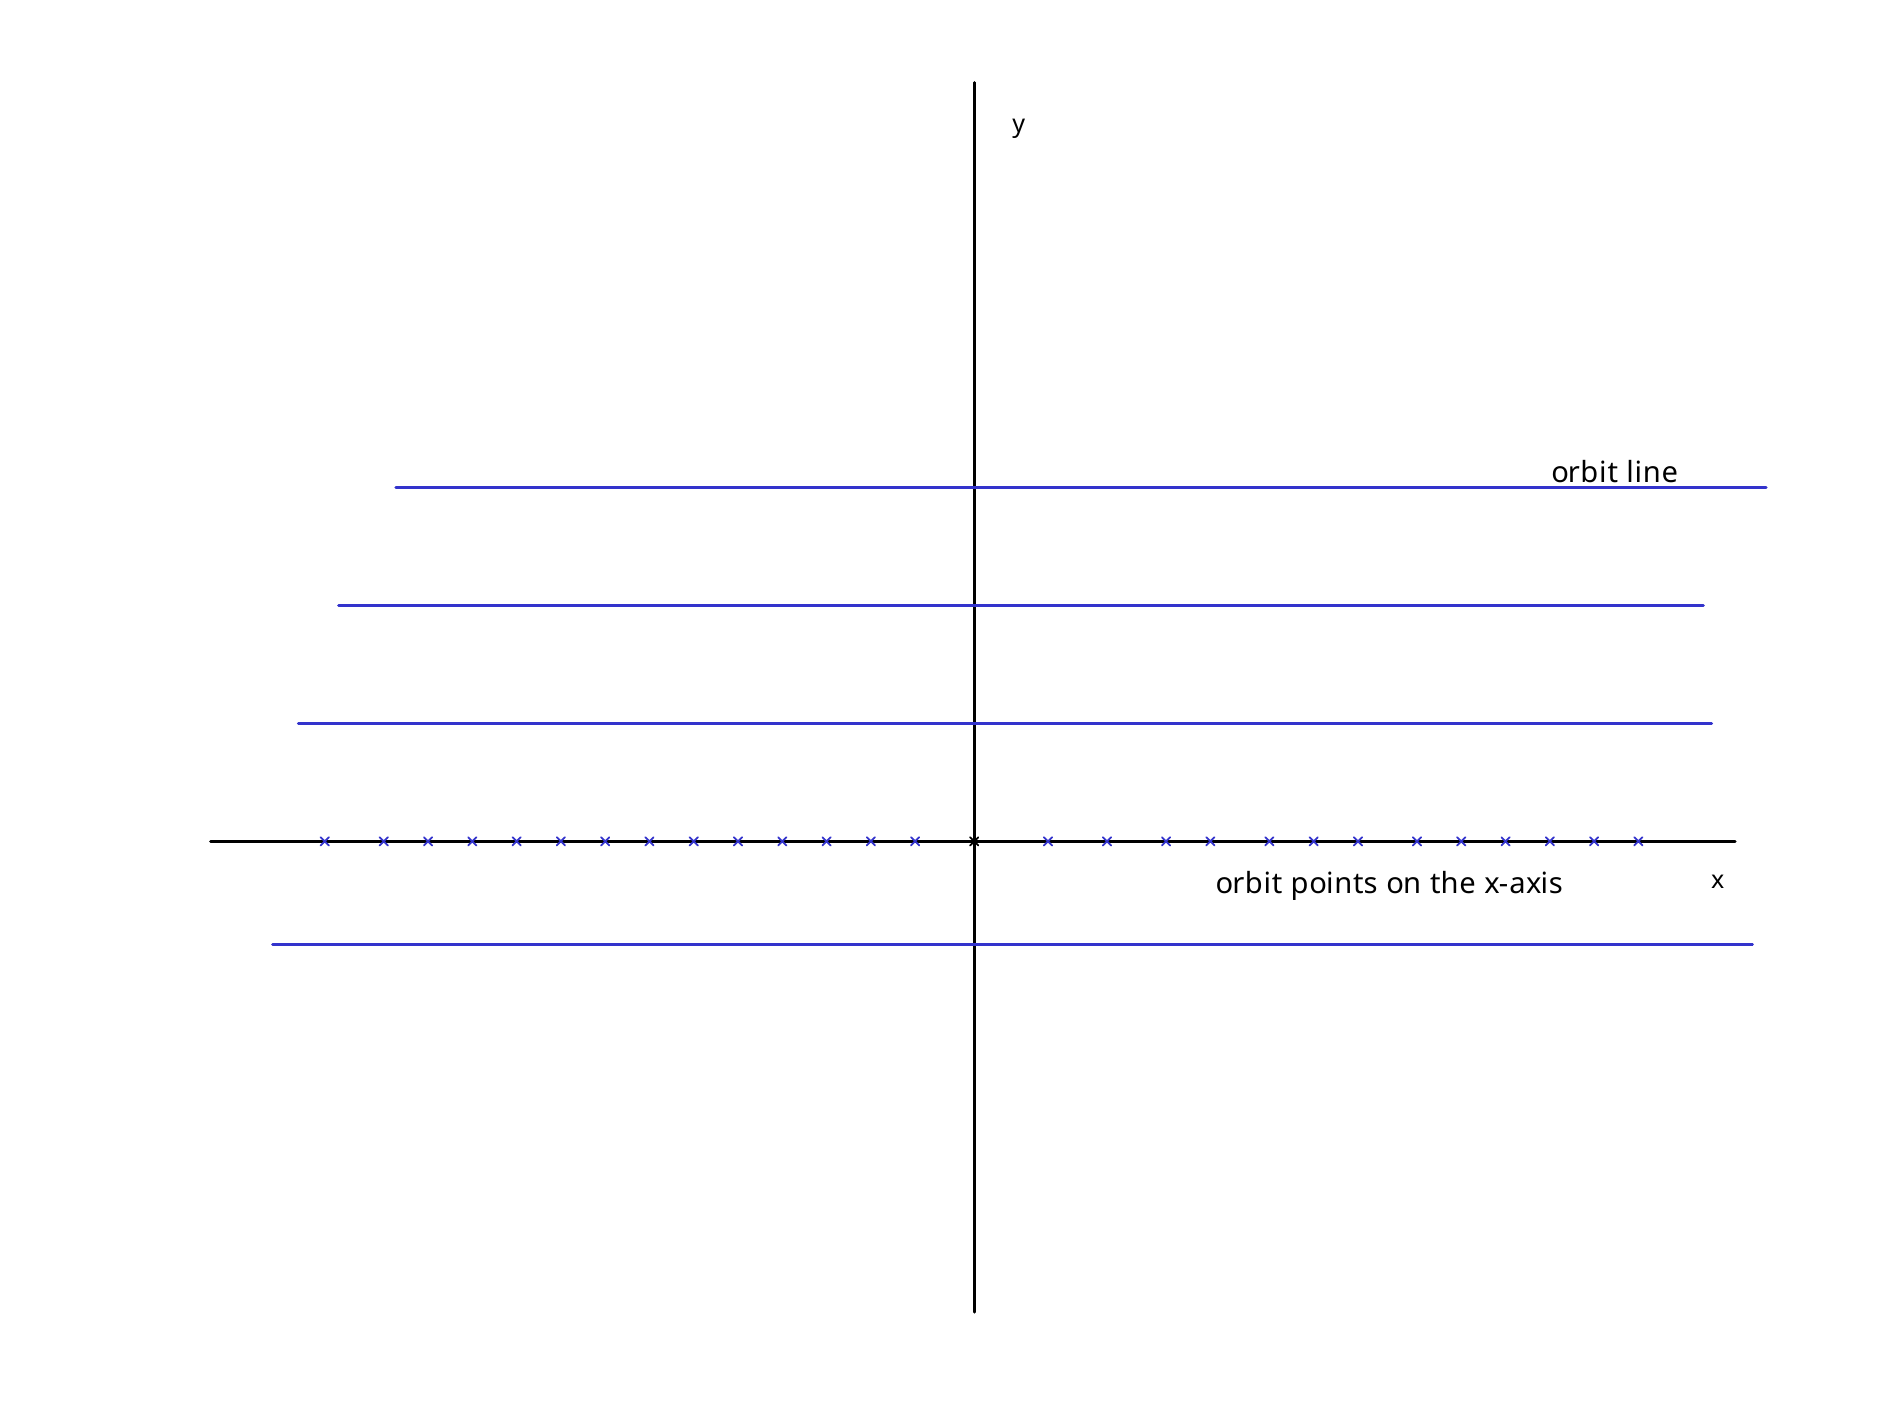
\includegraphics[width=0.95\textwidth]{N-orbits-in-R2-1.png}
    \end{center}
    \caption{The orbits of $N$ on $G/N$ correspond either to the horizontal lines parallel to the x-axis or to the individual points on the x-axis. }
    \label{fig:n-orbits-in-r2}
  \end{figure}

  But we can also identify the $x$-axis with $P/N$ by $\ipmatrix{a & b \\ 0 &
  a^{-1}}\ipmatrix{x \\ 0} = \ipmatrix{ax \\ 0}$. Therefore $f$ is also
  constant on $P$. So it follows that $v$ is $P$-invariant. And as we've seen
  in the \hyperref[sec:introduction]{intoduction}, we can identify $G/P$ with
  the real projective line and $P$ has a dense orbit in $G/P$ so $f$ is
  constant on $G$ and therefore $v$ is actually \G-invariant, contradicting our
  assumption.


%%%%%%%%%%%%%%%%%%%%%%%%%%%%%%%%%%%%%%%%%%%%%%%%%%%%%%%%%%%%%%%%%%%%%%%%%%%%%%%%

\hypertarget{proof-for-slnr}{%
  \subsection{Proof for \texorpdfstring{$SL(n, \mathbb{R})$}{SL(n, R)}}
\label{proof-for-slnr}}




  In this section we'll prove the statement for $G = \slnr$ and later show how
  the proof is extended to a general group \G. We begin just as for \sltr, by
  applying \hyperref[lemma]{lemma} \ref{lemma}. Thus it suffices to show that
  matrix coefficients vanish on $A \subset G$ to imply that they vanish on \G.

  Let $A \subset G$ be the subgroup of diagonal matrices. We denote the elements

  $$
  A \ni a := \begin{pmatrix}
    a_1 & & \\
        & \ddots & \\
        & & a_n
  \end{pmatrix}
  $$

  by $(a_1, \dots, a_n)$.

  To get an equivalent to the group $N$ from the earlier proof, we first define the group $B$, which has $1$ on the diagonal and $0$ everywhere but the first row.

  $$
    B \ni b := \begin{pmatrix}
      1 & b_{1,2} & & \cdots & & b_{1,n} \\
      0 & & &  & \\
      \vdots & & & \Id_{n-1} & \\
      0 & & & & \\
    \end{pmatrix}
  $$

  and write $b = (1, b_2, \dots, b_n)$, specifying only the first row.
  We now have analogues for $A$, $N$ and we set $H:=AB$. We will replicate the proof for \sltr on this group.
  In the case of $n = 2$, this reduces to \sltr and the above matrix to $N$ from the previous proof.

  Observe $B \cong \bbr^n$.
  These one-row spaces like $B$ are actually abelian normal subgroups.
  To see abelianness, decompose the matrix into $(\Id + b)(\Id +b') = \Id + \Id\cdot b + \Id\cdot b' + b\cdot b'$.
  Note that a b are nilpotent and by choosing the same row for our entries they
  ``miss'' each other during multiplication and so $b\cdot b' =0$. The rest then commutes
  due to commutativity of matrix addition.
  Similarly, we get that $A$ normalizes $B$: $aBa^{-1} = a(\Id + b)a^{-1} = \Id + aba^{-1}$.
  The last term will again be entirely in the first row and therefore the entire expression will be in $B$.
  Calculation shows $aba^{-1} = (1, a_1a_2^{-1}b_2, \dots, a_1a_n^{-1}b_n)$.

  The adjoint action on $\hat{\bbr}^{n-1}$ will be given by the same expression,
  replacing $b_i$ by the dual variables $\lambda_i$, $i = 2, \dots , n$.
  Therefore, if $E,\ F \subset \hat{\bbr}^{n-1}$ are
  compact subsets which are disjoint from the union of the hyperplanes $\lambda_i = 0$,
  $i = 2, \dots , n$ then for $a\in A$ outside a sufficiently large compact set, we have
  $a\cdot E \cap F = 0$.

  Therefore, as in \thref{thm:2.3.6} if $\mu$ assigns measure $0$ to the union of the hyperplanes $\lambda_i =0$ then all matrix coefficients vanish along $A$, which proves the theorem.

  It remains to analyse the case $\mu(\{\lambda_i=0\}) > 0$ and show that this is impossible.

  If $\mu(\{\lambda_i=0\}) > 0$, then the subgroup $B_i \subset B$, $B_i := \{b \in B\ |\ b_j=0 \text{ for } i\neq j\}$ leaves non-trivial vectors invariant.

  However $B_i \subset H_i \subset G$ where $H_i \cong \sltr$ as follows: the matrices in $H_i$ are those that have ones on the diagonal and zero elsewhere except for the index combinations $(1,1),\ (1,i),\ (i,1),\ (i,i)$.

  $$
  H_i = \begin{pmatrix}
    c_{11} & & c_{1i} & \\
           & \ddots & & \\
    c_{i1} & & c_{ii}&  \\
           & & & \ddots
  \end{pmatrix}
  $$

  From the proof for \sltr we know that $B_i$-invariant vectors imply $H_i$ invariant vectors. In particular $A_i = A \cap H_i$ has non-trivial invariant vectors.

  Let $W = \{v \in \hilb | \pi(a)v=v\}$. We show that \G leaves $W$ invariant.
  First, since $A_i \subset A$, $A$ abelean, $A$ leaves $W$ invariant. Now
  consider matrices $B_{kj}$ which have 1 along the diagonal and 0 elsewhere,
  except for the coefficient $(b_{kj})$. If $k\neq j$ and $j\neq i$ or $1$ then
  $B_{kj}$ commutes with $A_i$ and therefore leaves $W$ invariant. If
  $\{k,j\}\cap \{1,i\} \neq \emptyset$ then $A_i$ normaliyes $B_{kj}$.
  Therefore $A_iB_{kj}$ is isomorphic to $P$ such that $A_i$ corresponds to the
  diagonal matrices in $P$ and $B_{kj}$ corresponds to $N$. By
  \thref{cor:2.3.7} this case as well, leaves $W$ invariant.

  The proof finishes with the argument that if $W$ is \G-invariant, then the
  representation $\pi_W$ has $A_i \subset \text{kernel}(\pi_W)$. And because \G
  is simple this implies that $\text{kernel}(\pi_W) = G$, so that \G leaves all
  vectors in $W$ fixed, contradicting our assumptions.

  For the last paragraph, note that if \G is semisimple, the fact that
  $\dim(\text{kernel}(\pi_W)) >0$ contradicts the assumption that no simple
  factor of \G leaves bectors invariant.


%%%%%%%%%%%%%%%%%%%%%%%%%%%%%%%%%%%%%%%%%%%%%%%%%%%%%%%%%%%%%%%%%%%%%%%%%%%%%%%%


\hypertarget{proof-for-a-general-G}{%
\subsection{Proof for a general \texorpdfstring{$G$}{G}}\label{proof-for-a-general-G}}



   In concluding this section, we indicate the
   To conclude the proof, we show how to extend the argument to a general semisimple group.

   This follows essentially from the Iwasawa decomposition of a semisimple group.

   For detailed proof of the facts we're going to use, see \citeauthor{Hilgert2012}\cite{Hilgert2012} chapter 13.3 and in particular theorem 13.3.8.
   
   Let \G be semisimple and $\mathfrak{g}$ its associated Lie algebra, then 
   $$\frg = \frk + \fra + \frnn$$
   Then $G =KAN$ with $K=exp_G(\frk)$, $A=exp_G(\fra)$ and $N=exp_G(\frnn)$
   and there exists a basis of \frg such that the elements of $K$ are represented by orthogonal matrices, the elements of $A$ by diagonal matrices with positive entries, and the elements of $N$ are represented by unipotent matrices.

   By the same argument we made for \thref{lemma}, we can focus on the subgroup $B=AN$ and analyze it in the same way as the case for \slnr.


%%%%%%%%%%%%%%%%%%%%%%%%%%%%%%%%%%%%%%%%%%%%%%%%%%%%%%%%%%%%%%%%%%%%%%%%%%%%%%%%


\hypertarget{outro}{%
\section{Conclusion}\label{outro}}


  Now that we've proven the theorem, it's natural to ask what we do with it now.
  At first glance, the statement about matrix coefficients doesn't seem particularly useful,
  but recall from this \hyperref[the-connection-between-ergodicity-and-unitary-representations]{section}
  that we have a connection to invariant subsets of a possibly ergodic space.

  We have mentioned in the very beginning where we wanted to go with this, but let's recall it here.

  The problem we posed at the beginning is the following:

  \begin{problem}[When do closed subgroups act ergodically]
    Let \G be a semisimple Lie group and $S$ an ergodic \G-space. If $H\subset G$ is a closed subgroup, when is $H$ ergodic on $S$.
  \end{problem}

  We'll show how we can apply the theorem to this problem, mostly forgoing proofs.

  \begin{thm}[Zimmer 2.2.19, originally \citeauthor{Moore66}\cite{Moore66}]
    \label{thm:2.2.19}
     Let $G_i$ be semisimple, non-compact Lie groups and $G = \prod G_i$ and
     suppose \mpi is a unitary representation that has no invariant vectors of
     \G such that \mpi has no invariant vectors for each $\pi|G_i$. If $H
     \subset G$ is a closed subgroup and $\pi|H$ has non-trivial invariant
     vectors then $H$ is compact.
  \end{thm}

  \begin{pf}
    This follows immediately from then theorem because if $\pi|H$ has an invariant vector $v$, then the matrix coefficient $\inn{\pi(g)v,v}$ is identically 1 along $H$, and therefore $H$ is compact.
  \end{pf}


  By the theorem \thref{thm:2.2.17}, this is equivalent to the following:


  \begin{thm}[Zimmer 2.2.15]
    \label{thm:2.2.15}
    Let $G = \prod G_i$ be a finite product where each $G_i$ is a connected
    non-compact simple Lie group with finite center. Suppose $S$ is an
    irreducible ergodic \G-space with finite invariant measure. If $H \subset
    G$ is a closed non-compact subgroup, then $H$ is ergodic on $S$.
  \end{thm}

  For the case of spaces with finite invariant measure the established condition is exactly necessary and sufficient for ergodicity.

  Recall that the defition of a lattice specifies that the quotient $G/Gamma$ has finite measure. This means for actions on that space, searching for invariant vectors is exactly equivalent to establishing ergodicity.

  In conclusion we can put our results into the following statement:

  \begin{thm}[Zimmer 2.2.6, Moore's Ergodicity Theorem]
    \label{thm:2.2.6}
    Let $G = \prod G_i$ be a finite product where each $G_i$ is a connected
    non-compact simple Lie group with finite center. Let $\Gamma \subset G$ be
    an irreducible lattice. If $H \subset G$ is a closed subgroup and $H$ is
    not. compact, then H is ergodic on $G/\Gamma$.
  \end{thm}



  % TODO: def 2.2.4 needs to get in here somehow.

  % circle back to fractional linear transforms.
  % hyperbolas! 3 cases comp eucl and non-comp. if we want to go to infinity
  % and don't want boring examples, hyperbolic geometry is necessary.
  % fractional linear transforms. riemann sphere model?


%%%%%%%%%%%%%%%%%%%%%%%%%%%%%%%%%%%%%%%%%%%%%%%%%%%%%%%%%%%%%%%%%%%%%%%%%%%%%%%%



\cleardoublepage


\section{List of Theorems}
\theoremlisttype{allname}
\listtheorems{thm,lem}

\phantomsection
\addcontentsline{toc}{section}{List of Figures}
\listoffigures

\phantomsection
\addcontentsline{toc}{section}{Bibliography}
\printbibliography
\includepdf[pages={-}]{decl-of-originality-signed.pdf}

\end{document}
